\documentclass[11pt]{article}

\usepackage{natbib}
\usepackage{aas_macros}
\usepackage{hyperref}
% \usepackage{aasmacros}
% \usepackage{geometry}                % See geometry.pdf to learn the layout options. There are lots.
%\geometry{a4paper}                   % ... or a4paper or a5paper or ... 
%\geometry{landscape}                % Activate for for rotated page geometry
%\usepackage[parfill]{parskip}    % Activate to begin paragraphs with an empty line rather than an indent
\usepackage{graphicx}
\usepackage{amssymb}
%\usepackage{epstopdf}
%\DeclareGraphicsRule{.tif}{png}{.png}{`convert #1 `dirname #1`/`basename #1 .tif`.png}

\begin{document}

\begin{figure*}
    \centering
    \fbox{\includegraphics[width=0.8\textwidth]{NIRISS_AMI.png}}
    % \caption{Caption}
    % \label{fig:enter-label}
\end{figure*}

\title{Optical interferometry}
\author{Staff contact: Grant Kennedy}
\date{}                                           % Activate to display a given date or no date

\maketitle

\clearpage

\tableofcontents

\clearpage

\noindent\fbox{
\parbox{\textwidth}{
The goal of this experiment is to illustrate the main concepts of interferometry as used in astronomical observations. By the end you should understand three key things:
\begin{itemize}
    \item What interferometry is and conceptually how it works.
    \item Visibility, and how it relates to wavelength, baseline, and source size.
    \item How observations can infer spatial information about a source.
\end{itemize}
Showing that you understand these ideas in your report is recommended!
}
}

\section{Introduction}

One of the most famous physics experiments is Young's double slit experiment\footnote{For an introduction, \href{https://en.wikipedia.org/wiki/Double-slit_experiment}{Wikipedia} and \href{https://www.youtube.com/watch?v=A9tKncAdlHQ}{YouTube} are good places to start.}, where light from a single monochromatic point source passes through two slits and forms ``fringes'' on a screen or detector. The spacing of these fringes is $\lambda/b$, where $\lambda$ is the wavelength of the light, and $b$ the distance between the slits. The bright fringes are where the difference in path lengths from the two slits to the screen is an integer number of wavelengths, so the light constructively adds, and the dark fringes are where the paths differ by half of the wavelength of the light, and so cancel. This experiment has several \href{https://en.wikipedia.org/wiki/Double-slit_experiment}{remarkable properties}; it still works when photons are sent through one at a time, and also works for particles such as electrons.

There is an important question to ask of this experiment; what happens if the source is not a point? One reason to ask this question is that real sources are never really points, and have some finite size. For example, in the context of astronomy, while we can for most purposes consider stars to be point sources because their angular size is very small compared to the resolution of typical telescopes, given sufficient angular resolution this assumption is not true.

A finite source size fundamentally changes the double slit experiment as we normally encounter it. The simplest way to envisage an extended source is to add a second point source of equal brightness that is incoherent with the first. If we add this source at an angle $\lambda/(2b)$ away from the first, the two fringe patterns are $180^\circ$ out of phase so will cancel, leaving a uniformly illuminated detector with half of the peak brightness.

\clearpage

While either source would individually produce a set of fringes, together their fringes add to produce none, and this difference is the result of the spatial separation of the two sources. \textbf{That is, the double slit experiment therefore provides a means to infer spatial information about sources by measuring fringe patterns.} Here we will be concerned with the fringe amplitudes, which are also known as ``fringe visibilities'' or simply ``visibilities''. Though we will not be concerned with them here, the phases are also important, primarily giving information regarding spatial location (e.g. consider how the fringes in the single source case move as the source is moved to one side; the amplitude remains the same but the phase changes).

The first use of such an ``interferometer'' in astronomy was to measure the size of the moons of Jupiter \citep{1891PASP....3..274M,1891Natur..45..160M}, and 30 years later the technique was used to measure the diameter of another star \citep{1921ApJ....53..249M}. Interferometry is now a widely used technique in astrophysics, and is normally concerned with measuring the sizes of small objects, or with obtaining images of objects and structures that have relatively small angular scales.

% What does ``small'' mean here? As we saw above, when the separation between two point sources is $\lambda/(2b)$, the fringes disappear (the visibility is zero). The angular resolution of an interferometer is therefore defined as $\lambda/(2b)$, where $b$ is the distance between two telescopes, that serve the same purpose as the slits in the double slit experiment. Compare this to Rayleigh's criterion, $1.22 \lambda/D$, where $D$ is the diameter of the aperture or telescope. Now if $D$ and $b$ are similar the resolution of an interferometer and a normal ``single-dish'' telescope is similar. But there is one key difference; the space between the two telescopes of an interferometer can be empty, meaning that it is practically much easier and cheaper to make $b$ large (e.g. tens/hundreds of meters for optical wavelengths, and kilometers for millimeter wavelengths) than it is to make $D$ large. The largest single-dish telescopes we have are of order tens (optical) to hundreds (radio) of meters.

The key thing an interferometer does is allow us to make measurements on small angular scales, without constructing a single-dish telescope that would do so based on Rayleigh's criterion. In this experiment you will use exactly the same methods used in optical interferometry, just on a smaller scale.

As an example, the image on the front page shows a real-world example of an ``aperture mask'', as used by the \href{https://jwst-docs.stsci.edu/jwst-near-infrared-imager-and-slitless-spectrograph/niriss-observing-modes/niriss-aperture-masking-interferometry}{James Webb Space Telescope}. This has seven holes, but works exactly the same as 21 individual double-slit experiments done simultaneously.

The remainder of this document covers the background theory in a bit more detail (\S \ref{sec:theory}), followed by a quick connection with the real world of interferometry in \S \ref{sec:realworld}. The experimental setup is then described (\S \ref{sec:exp_setup}), and how to measure and model visibilities in sections \ref{sec:meas} and \ref{sec:models}. What you should actually attempt to measure during the lab sessions, and some suggested practical ways to work, are given in section \ref{sec:exp}.

\clearpage
\section{Theory}\label{sec:theory}

As outlined above, this experiment is little more than an extension of Young's double slit experiment. The only real difference is that we will be using an extended source that is incoherent. Typically the double slit experiment uses a coherent point source (e.g. a laser). Here the slits will also be replaced with pairs of holes, so instead of the usual one-dimensional picture, fringes are spread over a two-dimensional plane with an orientation that depends on the orientation of the holes. 

\begin{figure}[h]
    \centering
    \includegraphics[width=0.8\textwidth]{doc/youngs.png}
    \caption{Illustration of Young's double slit experiment (\emph{left}), and the resulting intensity image when two point sources are observed (\emph{right}). Credit: \citet{2003RPPh...66..789M}.}
    \label{fig:youngs}
\end{figure}

To recap the double slit experiment more formally, Figure \ref{fig:youngs} shows the expected fringe pattern for a point source at infinity and with slits that have a spacing $b$. In interferometry, this separation is commonly called a ``baseline''. We assume that we are observing light that has a limited range of wavelengths $\Delta \lambda$ that is centered on the mean wavelength $\lambda$. The fringe pattern then has a spacing of $\lambda/b$; this is the angle in radians between fringe peaks from the plane of the slits to the detector. The fringe pattern intensity $I$ is commonly written as
\begin{equation}\label{eq:fringepattern}
    I = 4 I_0 \cos^2 \frac{\delta}{2}
\end{equation}
where $I_0$ is the intensity that would have resulted from light passing through a single hole or slit, and where $\delta$ is the phase difference that results from the different path lengths from the slits to a given point on the detector.

Now consider a second source of equal brightness, with an angular separation from the first of $\lambda/(2b)$. The fringes produced by this source will be 180$^\circ$ out of phase compared to the fringes from the first source, so will cancel. Because we are considering an analogy with an astronomical observation, the two sources are expected to be incoherent because their spatial separation will typically be large (e.g. thousands of km apart on the surface of a star) and there is no reason to believe there is any laser-like behaviour that synchronises photon phases, so the phases of two photons coming from the two sources will have random phases with respect to each other. Thus, at any point on the detector we can simply add the intensity from the two independent fringe patterns (there is no sustained interference between the two patterns). For the case with the second source separated by $\lambda/(2b)$, the result is therefore no fringes at all, as shown in the right panel of Figure \ref{fig:youngs}. This disappearance of the fringes is how we define the resolution of an interferometer, while for single-dish (normal) telescopes with diameter $D$ it is the Rayleigh criterion of 1.22\,$\lambda/D$, for interferometers it is $\lambda/(2b)$.

\begin{figure}[h!]
    \centering
    \includegraphics[width=0.9\textwidth]{doc/coherence.png}
    \caption{Illustration of how the fringe pattern is altered by a finite range of wavelengths and an extended source size (assuming a baseline of 10\,cm). Each panel shows several of the fringe patterns that are being superimposed, which result in the overall pattern shown as the thicker black line. The top left panel shows the fringe pattern for a monochromatic point source, and the other panels show how the fringe amplitude is reduced. The top right shows the effect for a range of wavelengths in the `K' band (near 2.5\,$\mu$m). The lower left panel shows the effect for an extended source, and the lower right panel the combination of an extended source and range of wavelengths. Credit: \href{https://www.eso.org/sci/facilities/paranal/telescopes/vlti/tuto/tutorial_spatial_interferometry.pdf}{Andreas Glindemann/ESO}}
    \label{fig:coherence}
\end{figure}

In intermediate cases where a second source is less separated, e.g. at $\lambda/(4b)$, the fringe patterns do not add up to a constant, but the amplitude of the pattern is still reduced. The same behaviour is typically observed when the source is extended, e.g. a uniform disk such as a stellar surface, since this case can be considered as the summation of a series of point sources. This reduction in fringe amplitude is illustrated in Figure \ref{fig:coherence}, most importantly in the lower left panel which considers a finite continuous source. A finite range of wavelengths will also reduce the fringe amplitude, though in this experiment we will reduce this effect by using filters to restrict the range of wavelengths.

In interferometry we are primarily interested in the amplitude of the fringes formed on our detector. We characterise this amplitude with the ``visibility'', which is defined as
\begin{equation}
    V = \frac{I_{\rm max} - I_{\rm min}}{I_{\rm max} + I_{\rm min}} \, .
\end{equation}
Looking at Figure \ref{fig:coherence}, we can see that the fringes in the top left panel have $V=1$ (and in the left panel of Figure \ref{fig:youngs}). For resolved sources the visibility is lower, for example in the lower left panel the value is about 0.6. For the right panel in Figure \ref{fig:youngs} the visibility is zero. Depending on how we measure it, a finite wavelength range will also lower the visiblity, as can be understood from the top right panel in Figure \ref{fig:coherence}.

\clearpage

In general, the fringes are an indication of how well ``resolved'' a source is. An unresolved source will have strong fringes and a high visibility, but as the source becomes more extended the fringes weaken and the visibility drops. For continuous sources as we will be considering here, which are analogous to the surface of a star for example, when the source is larger than about $\lambda/(2b)$ the visibility drops to near zero. This can be understood as the image on the detector being the superposition of many fringes that have such a wide range of phases that the average is a constant.

\begin{figure}
    \centering
    \includegraphics[width=0.25\textwidth]{sky-fringes.pdf}
    \caption{Fringes projected on the sky; the fringe amplitude goes from -1 (black) to 1 (white), and $\lambda/(2b)=10$. A single source anywhere will produce a visibility amplitude of 1, but with different phases. A binary with one star at 0,0, and the other at 10,0 will produce a visibility of zero.}
    \label{fig:sky-fringes}
\end{figure}

A more quantitative way to understand the origin of the visibility is that it is equal to the integral of the fringes as projected on the sky multiplied by the source. That is, picture the sky with a two-dimensional sine wave plotted on top, as shown in Figure \ref{fig:sky-fringes}. For the binary example with separation $\lambda/2b$, one source is on the peak of a fringe (0,0), while the other is on a minimum (10,0), so the integral is zero. An extended source, e.g. a star, that spans many fringes (e.g. a diameter $\gtrsim$10) will have a low visibility (i.e. the integral over several cycles of a sinusoid is zero), but one that is smaller than the fringe spacing will have a high visibility.

When making a measurement, we normally change the resolution of our instrument (i.e. the fringe spacing), either by changing the wavelength $\lambda$ or the baseline length $b$. This can be pictured as varying the fringe spacing on the sky. A typical measurement therefore consists of making visibility measurements for a range of wavelengths and baseline lengths, and using these to infer spatial information about our source.

Note that one pair of baselines, we are only measuring the source size along an axis parallel with the baseline vector. For sources that are not rotationally symmetric, we can address this by rotating our baselines to a different angle with respect to the source and taking more measurements.

\subsection{Visibility functions}

Mathematically, we can write down the expected behaviour of the visibility as a function of baseline and wavelength for a few different source geometries. Some more detail on where these come from is given in \citet[][e.g. Fig 2.13]{2011psi..book.....G}. Mathematically, the connection between the sky and the visibilities is the ``\href{https://en.wikipedia.org/wiki/Van_Cittert%E2%80%93Zernike_theorem}{van Cittert-Zernike Theorem}'', which states that the Fourier transform of the intensity distribution function of a distant, incoherent source is equal to its complex visibility. With the measurements in this lab, we are sampling the visibility at specific spatial frequencies (i.e. at points in the FT of the sky image that correspond to specific $b/\lambda$).

The visibility for a binary source is perhaps not too surprising, we saw above that $V=1$ when their separation is zero, and $V=0$ when their separation is $\lambda/(2b)$. Based on the idea of projecting fringes on the sky, $V$ therefore varies sinusoidally in between. For an equal brightness binary with separation $s$, the visibility is
\begin{equation}
    V^2_{\rm binary} = \frac{1 + \cos ( 2 \pi s b / \lambda )}{2} \, .
\end{equation}

For an extended uniform circular source of diameter $\theta$ as a function of baseline length the visibility is
\begin{equation}\label{eq:uniform}
    V_{\rm uniform} =  \left\vert \frac{2 J_1(\pi \theta b / \lambda)}{\pi \theta b / \lambda} \right\vert \, ,
\end{equation}
where $J_1$ is a first order Bessel function. We take the absolute value because here we are not concerned with the phases (i.e. a negative visibility corresponds to a 180$^\circ$ difference in phase compared to a positive one). Connecting this result to the van Cittert-Zernike theorem, recall that the Fourier transform of a 1d top hat function is $\sin(x)/x$; equation (\ref{eq:uniform}) is simply the same result in 2d.

\begin{figure}
    \centering
    \includegraphics[width=0.8\textwidth]{doc/uniform_vis.png}
    \caption{Absolute visibility for a uniform source of 2\,mm diameter at a distance of 7\,m. For optical wavelengths the baselines are of order millimeters.}
    \label{fig:uniformvis}
\end{figure}

Equation (\ref{eq:uniform}) is the visibility function that you will need for this experiment. To visualise either, the independent variable you are controlling is $b/\lambda$, so this should be the x-axis, and visibility is the quantity you are measuring, so this is the y-axis. As described above the uniform source therefore has decreasing visibility with increasing $b/\lambda$.

An example visibility curve for a uniform source is shown in Figure \ref{fig:uniformvis}. The y-axis plots the absolute value, as we only measure visibility in this experiment as a positive value (squared visibility is also commonly used). This plot is for a 2\,mm diameter source at 7\,m, which is similar to what you will use for this experiment. Likewise, the baselines are similar to this experiment, e.g. a 1\,mm baseline at 500\,nm is $b/\lambda=2000$.

\clearpage
\section{The real world}\label{sec:realworld}

There are two main connections to the real world of interferometry, but conceptually everything is exactly the same as this experiment. The first is the case where each pair of holes is two telescopes, an example is the \href{https://en.wikipedia.org/wiki/CHARA_array}{CHARA} array on Mt Wilson in California. This facility is a series of individual telescopes, whose light is brought together on an optical bench and interfered. The baselines are of order tens of meters, so the angular resolution is better than even the largest optical single-mirror telescopes.
% Compared to this experiment there are many complications, for example to properly interfere the light from pairs of telescopes the different path lengths from each telescope must be accounted for, for which there is a large temperature-controlled room with delay lines.
CHARA has measured the diameter and shape of \href{https://www.chara.gsu.edu/science-highlights/rapid-rotators}{rotationally flattened stars} \citep[e.g.][]{2011ApJ...732...68C}, analogous to the part of this experiment that uses the ``Saturn'' source.

\begin{figure}
    \centering
    \includegraphics{doc/NIRISS_AMI.png}
    \caption{A prototype of the non-redundant mask on JWST. Credit: \href{https://jwst-docs.stsci.edu/jwst-near-infrared-imager-and-slitless-spectrograph/niriss-observing-modes/niriss-aperture-masking-interferometry}{JWST}.}
    \label{fig:ami}
\end{figure}

Another analogue of this lab experiment is even more closely related, called ``aperture masking''. In this case, an optical element with a number of holes (the ``mask'') is placed in the optical path. The light passes through these holes and interferes, creating a fringe pattern that can be interpreted with a Fourier transform. That is, with this lab you are doing aperture masking, with the only difference being that the masks used for astrophysics have a greater number of holes and the telescopes are bigger. One example is the \href{https://jwst-docs.stsci.edu/jwst-near-infrared-imager-and-slitless-spectrograph/niriss-observing-modes/niriss-aperture-masking-interferometry}{James Webb Space Telescope}, for which one of the instruments uses aperture masking. An example mask is shown in Figure \ref{fig:ami}. This mask is ``non-redundant'', meaning that no two of the 21 baselines are the same.

\clearpage
\section{Experimental setup}\label{sec:exp_setup}

This lab has an intentionally simple setup; the goal is to show how one can construct an interferometer from a standard telescope with minor and straightforward modifications. You will also use some software that is outlined below. Some parts are a bit fiddly, this is also intentional; real experiments do require some precision from the scientists! The key physical pieces of equipment are (see the Appendix for some photos):
\begin{itemize}
    \item The physics lab, which in the microprocessors room you can take to be 992\,cm long wall to wall. You can find the distance between the aperture and the front of the telescope by measuring their distances from the walls with a ruler.
    \item Telescope, this is a 90mm \href{https://www.celestron.com/products/c90-mak-spotting-scope#description}{Celestron} C90 Maksutov-Cassegrain ``spotter'' telescope, which is mounted to the bench and can be flipped up or down. Down is probably easier, but check the path across the lab is clear.
    \item CMOS detector and USB cable. Some information on the detector is \href{https://www.qhyccd.com/qhy5l-ii-planetary-guiding-camera/}{here}.
    \item Lens cap with a small hole, this holds the tokens with the pairs of holes (baselines).
    \item Baseline tokens, these have small (0.3\,mm) holes drilled in pairs with a range of separations. These have spacings that are 0.6, 1, 2, 3, and 4\,mm. There is also a 3-hole token, with holes at 0.5 and 1\,mm separation at right angles (so the third baseline is $\sqrt{0.5^2 + 1^2}$\,mm).
    \item Light source. This is a USB-powered LED, and there are some bike lights as backup. The bike lights are much brighter (i.e. exposure times are shorter), but the batteries do not last very long.
    \item Aperture tokens, these go in front of the light source and are what we observe. The main one for this experiment has a single 2\,mm diameter hole. There is also `Saturn' which has a 4\,mm hole and two 2\,mm holes (outer size $4 \times 6$\,mm).
    \item Filters, used to change the wavelength of the source. You may take the mean wavelengths of these to be 448, 530, and 638\,nm for B, G, and R respectively. More detailed information on the filter response is \href{https://www.firstlightoptics.com/rgb-filters-filter-sets/zwo-2-lrgb-filter-set.html}{here}.
    \item Miscellaneous fittings to mount the light source, aperture tokens, and filters.
    \item An ITS (lab) computer near the telescope, plug the CMOS into this one.
\end{itemize}

\subsection{Image capture software}\label{sec:software}

The software for this experiment is \href{http://www.firecapture.de/}{\texttt{FireCapture}}; it is an open source code primarily designed for amateur astronomers, and provides a friendly and easy to use interface for viewing images from the detector in real time, and allows saving of images in various formats.

A copy of the software should exist in \texttt{C:} on the computer near where the telescope is set up. To run it, find your way down the file heirarchy to the \texttt{FireCapture} application and double-click to run it. You will probably be prompted to do some setup when you run \texttt{FireCapture} for the first time. Click the ``first time'' option; for most settings just leave the default, but select a new folder in which to save data on the ``capture'' options page. It would make sense to make another folder, e.g. \texttt{H://Interferometry/Data} for this, and if you use \texttt{H://} drive, you will have access to this from any other ITS machine.

A preferences file is saved in \texttt{C://Users/uXXXXXXX/FireCapture}. If you have problems, e.g. with the software crashing, try deleting this preferences folder and restarting \texttt{FireCapture}.

After the setup the software will go to a ``dummy camera'' that shows an image of Jupiter. Quit, and restart \texttt{FireCapture} when you have connected the detector (see setup steps below), at which point you should be prompted to select a detector, select \texttt{QHY}.

\begin{figure}[h]
    \centering
    \includegraphics[width=1\textwidth]{doc/fc.png}
    \caption{Screenshot of the \texttt{FireCapture} software running. The detector image is in the main panel, and various controls are in the left column.}
    \label{fig:fc}
\end{figure}

You will not need most of the options available in \texttt{FireCapture}. The main one in terms of obtaining images on screen is the exposure time (under ``control''); you will need to experiment, but values of about 1\,s are likely to be about right. You will need to alter the range that the exposure slider covers with the `X - Y ms' button to access a wide range of exposure times, or enter numbers by hand. The exposure time needed will however depend on what value you select for the gain. Higher gain images will require shorter exposures so be convenient when setting up, but will be noisier and introduce other artefacts, so it is better to take longer exposures at lower gain for measurements. Some gain is OK, you should not ever need exposures longer than a few seconds, and if the images don't have obvious artefacts that change with gain level (e.g. stripes) then the gain level is likely OK. You will know the exposure is appropriate when you have a clear image visible on screen that is not too noisy, and this image is not saturated (the ``histogram'' panel may help here).

You can see the values returned by the detector by moving the mouse over the image and looking at the `Pixel' number in the histogram panel. These are digital units from the detector that go up to 255, which you can take to be proportional to the flux (e.g. in W\,m$^{-2}$). You should aim to have the peak somewhere below 255 so the image is not saturated, peak counts anywhere above 150-200 are likely to result in a good image.

There are some options above the image to set how the image is displayed, e.g. zoom, which you may wish to play with. In particular, the field of view may not initially be maximal; this can be changed by selecting ``Max'' rather than ``ROI'' (which is a definable sub-section of the detector). You can also optionally bin the images (average $2 \times 2$ sets of pixels), this will increase the signal to noise, but be careful not to degrade the image too much for longer baselines (shorter wavelength fringes).

The other important control is how images are saved (under ``capture''); for this you need to specify a directory in which to save images (if you didn't already at startup), a file format (select ``FIT''), and a number of frames to save under ``limit'' (just one, since you will hit save manually each time you change the baseline token, filter, etc.). You can turn off the default behaviour that files are saved in their own subfolders by opening the `settings' window and un-ticking `Auto-create subfolders'.

You can optionally save a ``dark frame'' (one of the small buttons between the main image and the left column of controls). For this cover the front of the telescope (putting your hand in front of the baseline token would suffice), and \texttt{FireCapture} will take an image that will be subtracted off subsequent images. The goal is that this dark image will contain any ``hot'' (permanently defective) detector pixels and other detector artefacts, and by subtracting them these pixels will not be visible in the final images. Ideally your dark frame will have the same settings as the images it is being subtracted from, as different settings (gain in particular) will result in different artefacts.

\subsection{Python code}

There are a few pieces of python code, \texttt{widget.py} and some jupyter notebooks, to use in this experiment, all of which are on \href{https://github.com/drgmk/px-interferometry}{GitHub}. These are described later.

\clearpage

\subsection{Setup}\label{sec:setup}

Setting up the experiment is reasonably simple but takes some finesse, the aim being to have the telescope pointed at the aperture and the light source carefully aligned behind it. You will may find the setup quite difficult the first time, but typically the second time is many times faster!

Photos of the setup at either end of the lab are in the Appendix. While having the telescope properly focused will aid the setup, it's not actually critical for observing the fringes. A suggested series of steps to get your first set up fringes is as follows:

\begin{enumerate}
    % \item Plug the light source in to charge. The battery should last for a few hours, so it's best to turn it off and charge it when you're not using it.
    \item Ensure the telescope is in place (no tokens needed yet).
    \item Insert the CMOS detector into the rear of the telescope and (gently) tighten the screws to keep it in place.
    \item Connect the CMOS detector to the computer with the USB cable.
    \item Open the image capture software (see \ref{sec:software}). The detector should be automatically recognised (click ``QHY'' if not) and an image appear on screen. Test whether the detector is working by waving your hand in front of the telescope to vary the amount of light coming in. Check that ``Max'' rather then ``ROI'' is selected in Image box of \texttt{FireCapture} so you are seeing the entire detector.
    \item Set up the light source at the other end of the lab using the mounting kit (see example image in the Appendix). Aiming the light at the telescope is not particularly critical, but better alignment will give a more uniform surface brightness. It is easier to do these steps with the light off initially, but then turn it on and play with the LED orientation until the surface brightness is fairly uniform (you will need short exposures, low gain, and the lens cap on to avoid saturating the detector).
    \item Remove the telescope lens cap and set up the focus and pointing. The telescope is fixed, so you will need to adjust the location of the light until it appears near the center of the detector image. You will simultaneously need to adjust the exposure time and focus so you know what you are pointing at. If you think the pointing is a long way off, you may find it helpful to hold a large object (e.g. a book) in front of the token to figure out where you need to point. You should end up with an in focus image of the light source near the center of the detector.
    \item You may find it useful to orient the detector correctly, e.g. by placing a piece of paper near the source with an upwards pointing arrow on it, and rotating the detector so that the image on screen matches it. The orientation does not matter for rotationally symmetric sources.
    % \item Check the light source has a reasonably uniform surface brightness. You can test this by turning the light on and taking very short exposure images (perhaps with a filter to avoid saturation), and moving the source to get a reasonably uniformly bright disc.
    \item Now set up the aperture token with further mounting kit, ensuring the the surface normal of the token is pointing towards the telescope. You may find it helpful to note where in the image the center of the light is in \texttt{FireCapture} with the mouse cursor, and to then place the center of the aperture at this pixel.
    \item You can further check the aperture/source alignment by turning the light on and decreasing the exposure time enough to see the source without too much saturation, and verify that the source is centered behind the aperture and that the aperture is illuminated uniformly. Some examples are shown in Figure \ref{fig:img_setup}. Non-uniform illumination can result in unexpected results because the source size is not actually the size of the aperture, so this step is very important! You can  put the lens cap on the telescope with no baseline token to decrease the flux enough to image the aperture without saturation.
    \item Insert one of the baseline tokens into the lens cap, preferably one of the shorter baselines. You should now see fringes on the detector with an image similar to Figure \ref{fig:det-img}, though may need to alter the exposure time. A few seconds should be enough, though this will depend on gain and the light source. The fringes do not need to be perfectly centered on the detector; as long as the visible PSF is within the image the results will be OK.
    \item Finally, you can sanity check your setup by trying several different baseline tokens. Figure \ref{fig:uniformvis} shows an example visibility curve for parameters that are similar to the 2\,mm aperture; you can test whether you are likely to get a sensible aperture diameter by doing a quick visibility estimate for a few baselines/filters (i.e. $b/\lambda$) using the on-screen cursor to measure peak/trough counts.
\end{enumerate}

If all of this setup has gone well, you are now ready to start!

\clearpage
\section{Measuring visibilities}\label{sec:meas}

The key measurement in this experiment is of the fringe visibility. In the images this is essentially how strong the fringes are; if their amplitude covers the full range from peak to the background level the visibility is high (i.e. near 1), and if they are barely visible then the visibility is low (i.e. near zero).

\begin{figure}[h]
    \centering
    \includegraphics[width=0.8\textwidth]{doc/det-img.png}
    \caption{Example image. The broad circular envelope is the PSF, on which the fringes are superimposed. The small dots are artefacts from dust somewhere in the optical path, likely on the detector.}
    \label{fig:det-img}
\end{figure}

There are three components that contribute to an image, an example is shown in Figure \ref{fig:det-img}:
\begin{itemize}
    \item background; this is contributed by any stray light that reaches the detector, plus any intrinsic level attributed to the detector itself
    \item point spread function (PSF); this is the broad overall shape of the signal on the detector and is approximately Gaussian (but is really an Airy disk described by a Bessell function), and is set by the size of the individual holes in the baseline tokens. Smaller holes yield a larger diffraction pattern, and vice versa.
    \item fringes; this is the wavy pattern resulting from the pair of holes, the 2d version of the fringes from the experiment when done in 1d (e.g. with slits). The fringe orientation is set by the orientation of the holes (the fringes are perpendicular to a line between the holes), so can be used to quantify the orientation of the baseline token.
\end{itemize}
The goal in making a measurement is to subtract (or otherwise account for) the background, and make a measurement of the fringe visibility, which ideally takes the shape of the PSF into account.

The simplest method for obtaining a visibility measurement would be to use the cursor in \texttt{FireCapture} to measure the background level somewhere away from the PSF, take peak and trough measurements for the fringes, subtract the background level from these, and then compute the visibility.

A more complex, but more reliable method, is to use the supplied python widget (\texttt{widget.py}); this code models the above components of the detector image to come up with a parameterised fit to the data, from which the visibility can be extracted. It can also make a visibility measurement using a Fourier transform.

There is no ``correct'' method here, and each method has its own problems. The image model can fit poorly and not minimise well for longer baselines, and so be tedious to tune. The Fourier method can be less reliable and is influenced by various factors, e.g. noisy images and image size (see Fourier example notebook). You should experiment, for example making measurements with all three methods and comparing the results. You should also consider how to incorporate uncertainties.

\subsection{Using \texttt{widget.py}}\label{sec:widget}

This code brings up an interactive window that allows a parameterised fit to a detector image, and which will output the model parameters, including the visibility and baseline angle (with respect to the detector, whose orientation depends on how you insert it into the telescope). The code itself exists on github, you can download it from
\href{https://github.com/drgmk/px-interferometry}{https://github.com/drgmk/px-interferometry}.

To run the python widget you can use either a system or python terminal (see \ref{sec:widget_ipython} for the latter).

To run the widget from the shell directly, open the \texttt{WinPython PowerShell Prompt} from \texttt{C:}, there should be a \texttt{WinPython} install with a name like \texttt{WinPython-interferometry} (the default one is missing packages and will not work). This should exist on the computer the CMOS is connected to, and the other computer along the same end wall. You can make things easier by then changing directory (e.g. \texttt{cd H:\textbackslash Interferometry\textbackslash Data}) so that you are executing the code somewhere close to the data. To run the widget use something like (assuming here you are in the \texttt{px-interferometry} folder, and there is a data folder one level up)
\begin{verbatim}
    python widget.py ../data/filename.FIT -n 2
\end{verbatim}
The paths you enter will depend on where you run the command from, where you put \texttt{widget.py}, and where you save the data. A useful way to type these commands out is to use `tab completion'; start typing the path and hit the TAB key, which will fill out the rest of that part of the path (assuming it exists).

The final argument (here 2) does $2 \times 2$ averaging to make the array for the image smaller so the fitting code runs faster. You could try 4 or higher, but if you average too much the detail in the image will be lost and the fit will be poor. A suggested approach is to use 4, but go to 2 if the fringes are very close together and the fit is not converging as well as you expect.

On running the widget a window will pop up with the image (FITS file), a model, an image of the residuals (image-model), and a cut through the center of the image perpendicular to the fringes in the model. The model has the three components noted above, with the additional feature that the fringes account for a finite bandwidth so lose coherence away from the center somewhat. It uses a Gaussian instead of a Bessel function for the PSF by default; this is less accurate but much faster to compute. You could try using the Bessell function to improve the fits by adding the argument \texttt{-b}, though the results should be adequate with a Gaussian.
\begin{figure}[h!]
    \centering
    \includegraphics[width=1\textwidth]{widget.png}
    \caption{Example widget window. The top left panel shows the FITS image that is being fit. The top right shows the current model. The lower left shows the image-model residuals, and the lower right shows a cut through the image that is perpendicular to the model fringes (blue line), and the same cut through the model (orange line). This example shows the initial guess, so the model does not fit the image very well.}
    \label{fig:widget}
\end{figure}

The code will make an initial attempt to estimate the model parameters, see Figure \ref{fig:widget} for an example. The goal is then to improve the fit, which will almost certainly require some interaction. This works by moving the mouse cursor to a location on the image (top left panel), pressing a key on the keyboard to change some parameter, and repeating until the model is reasonably good. Details regarding keys can be found in the \texttt{widget.py} script and on the GitHub page. The fit can then be minimised (optimised) by pressing the \texttt{m} key. The residual plot may never look perfectly smooth, but the more uniform this image appears, particularly in terms of the residual fringe amplitures, the better the fit. An example of a good fit is shown in Figure \ref{fig:widget2} (which also shows the difference between Gaussian and Bessel functions).

The results can be saved into a \texttt{numpy} save file with \texttt{S}, but the visibility is also shown as a number in the lower right panel. The advantage of saving your results in a file is that you can speed up the extraction, fitting, and plotting of the results with a text file with the measurement details. See the visibility notebook for an example.

\begin{figure}[h]
    \centering
    \includegraphics[width=0.49\textwidth]{widget2.png}
    \includegraphics[width=0.49\textwidth]{widget3.png}
    \caption{Example widget windows with a good model fit to the data. In the left panel the PSF model is Gaussian, so still not a very good match to the overall envelope of flux. In the right panel the Airy disk is modelled properly with a Bessel function, with much better results (but note that the visibility is the same in both cases).}
    \label{fig:widget2}
\end{figure}

\subsection{Fourier components}\label{sec:fourier}

The images obtained in this experiment are relatively simple, in that they have the three components of background, PSF, and fringes described above. This simplicity makes it possible to obtain information by Fourier transforming the images. We first subtract the background, so there are only two components. The Fourier transform then has only a broad PSF, and the narrower fringes, or thinking in terms of frequencies, some low frequencies that correspond to the PSF, and a single higher frequency that describes the fringes.

\begin{figure}[h]
    \centering
   \includegraphics[width=1\textwidth]{widget-fourier.png}
    \caption{Example widget window with the Fourier option turned on. The visibility at the location of the `+' in the lower right panel is given in the legend.}
    \label{fig:widget-f}
\end{figure}

The result of Fourier transforming an image is shown in Figure \ref{fig:widget-f}. This version of the window can be obtained with the same call to \texttt{widget.py} or \texttt{widget.fit\_fringes()}, but with an extra argument. In the shell case, adding a \texttt{-f}  will invoke the Fourier panels. In the python terminal, adding \texttt{fourier=True} to \texttt{fit\_fringes()} is needed.

The modified image used in the Fourier transform is shown in the top right panel. If the background is low then this image will look identical to the top left one. The lower right panel shows a zoom in of the Fourier transform (the absolute value, here we will not use the phases associated with each frequency). It is an image, because the data are 2d, and the axes are such that the lowest frequencies are represented by pixels at the image center, and more distant pixels are increasingly high frequencies. The highest peak, at the center of the image corresponds to the overall PSF, and the two secondary peaks are the fringes. The orientation of the secondary peaks depends on the angle the fringes are at in the image. The fringes are represented by two peaks because both correspond to the same frequency and orientation.

The peaks for the PSF and fringes in the Fourier transform tell us how much power is in each component, and importantly, the peak for the fringe component is proportional to the visibility. The only thing to account for is how strong this peak is relative to the PSF peak, so we first scale the Fourier transform so that the peak in the center for the PSF is equal to 1. Then the visibility for a fringe component is $n_{\rm holes}$ times the peak value for that component. To understand why, picture just one component peak, then without the PSF component the image would be a localised sinusoid with positive and negative values. If the PSF component were added with the same peak value the image would then be all positive and look like the data in Figure \ref{fig:widget-f}. But if a second fringe component peak is present, the power in these peaks must be lower to get the same image because they add, so the peak value for the fringe component peaks should be halved. Thus, for visibility=1 and two holes, the peak value for the fringe component peaks is 0.5. If we had multiple sets of fringes, we could use a Fourier transform to decompose an image into its Fourier components (i.e. one for each baseline) and measure multiple visibilities at once. This is how the JWST and other aperture masks are used.

It is not straightforward to automatically identify the secondary Fourier peak, particularly at low visibilities, so \texttt{widget.py} uses the model to identify the appropriate pixel. This therefore requires a good fit to the fringes (which you will be aiming for anyway), or that you manually find the secondary peak using the cursor. If you hit `S' when using \texttt{widget.py} with the Fourier option, a file with the Fourier-based visibility will also be saved.

You can explore how the Fourier transform behaves for individual components in the images with the `fourier' notebook in the \texttt{px-interferometry} package.

Practically, visibility measurements with the Fourier method are more susceptible to low quality data, e.g. if the signal to noise ratio is low background image artefacts can influence the results (e.g. striping at high detector gain). Longer exposures with lower gain should yield better results. 

\section{Fitting models to visibilities}\label{sec:models}

Given a set of visibilities for a range of baselines and filters, a model (e.g. equation \ref{eq:uniform}) can be fit and a source diameter determined. An example jupyter notebook, which can be run using Noteable (link on moodle page), will guide you through this. For running jupyter notebooks on the lab ITS machines, see section \ref{sec:jupyter_its}, though this is not recommended since uploading images is tedious.

\clearpage

\section{The experiment}\label{sec:exp}

There are many possible measurements that could be made with this experimental setup. The two key ones you should do are:
\begin{itemize}
    \item Demonstrate the effect of bandwidth on coherence. This simply means exploring how the images depend on the filters used. No filter means that the bandwidth (range of wavelengths) is greater, so as in Figure \ref{fig:coherence}, the visibility is lower. By placing a filter in the light path, the fringe amplitude should increase. The spacing between fringe peaks should change with the filter wavelength.
    % First, estimate the bandwidth of the detector with no filter in place. This means estimating where the fringes become incoherent (e.g. after $n \times \lambda/b$ as in Fig. \ref{fig:coherence}), which then means the bandwidth is approximately $\lambda/(2n)$, where $\lambda$ is the mean wavelength of the band. You can derive this result from $(n-1/4)\lambda_1/b = (n+1/4)\lambda_2/b$. You will need to choose a baseline token that results in enough fringes to see this effect, but still has a significant visibility. Show that this coherence problem is significantly reduced when the filters are used.
    \item Measure the angular size of a circular source, the 2mm aperture token is the best choice. This means taking visibility measurements with multiple baselines and filters to cover enough range in $b/\lambda$ to constrain the source angular size. Because the source is circular the baseline orientation does not matter. You will need to consider how to estimate uncertainties (see `visibilities' notebook for an empirical method), and experiment with variables such as exposure time to get reliable results. If you use the Fourier option when fitting the fringes and save the results with `S', you will automatically have the Fourier visibilities for the next part below.
    % \item Verify the expected visibility variation with baseline for a binary source. A binary source that is too wide will be resolved out on even the shortest baselines, so a closer binary source is better. In this part you will need to ensure that the baseline holes have close to the same orientation as the binary. 
\end{itemize}

Beyond these some possible options are to:
\begin{itemize}
    \item Try repeating the source size measurement, but using visibilities from the Fourier transform (see section \ref{sec:fourier}). Compare your results from the image-fitting and Fourier methods, if one seems much worse, why?
    \item Use the three-hole baseline token to take some measurements for the 2mm source. This would involve using Fourier transforms as simultaneously fitting multiple fringes will be difficult. See `3\_hole' notebook for some guidance and an example. Once set up this part can be fairly quick, so try again for another source.
    \item Use the above method to characterise the shape of a non-rotationally symmetric source. This would involve the same method as for the sources above, but in addition rotating the baseline with respect to the source to measure the size as a function of baseline rotation. The `Saturn' source is slightly larger than the LED in the light source, so diffusing the light behind the aperture with the lens cap case will help. You may need to be inventive in how you hold the case in place. It's also likely that the USB-mounted LED is not bright enough; the demonstrator can supply the bike light if necessary, which is much brighter.
\end{itemize}

\subsection{Basic procedure}

The basic procedure for this experiment is to set things up as you desire and verify the setup is working visually using the image on the screen. Always take particular care with the setup, \textbf{especially uniform illumination of the aperture}, as this is the most common source of unexpected results (typically a smaller than expected aperture diameter). As noted above in section \ref{sec:setup}, sanity checking your visibilities in real time for a few baselines is worthwhile.

Images are then saved for some baseline and filter combinations to cover enough $b/\lambda$ space. The resulting images are then analysed with \texttt{widget.py} to obtain visibility measurements, and these visibilities are then used in concert with the baseline length and filter wavelength information to obtain a source diameter.

In doing all this you will need to keep track of files, what each was for, etc.. Saving files in separate folders for each part of the experiment will help, and of course keeping some records in a log book will be essential for your report.

Practically, you may find it expedient to work as a team, with one person changing filters at the source end, one person changing baseline tokens and operating \texttt{FireCapture} to save files in some systematic way, and one person fitting saved images to extract visibilities on another computer (one person can be logged into multiple computers, allowing the second person to access the newly saved files in \texttt{H:} from another lab machine).

The result would typically be a plot of visibility vs. $b/\lambda$, and a fit to the relevant theoretical curve to obtain an estimate of the source aperture size (i.e. similar to Fig. \ref{fig:uniformvis}). An example jupyter notebook for fitting a visibility function to data is included in Noteable, and in the \texttt{px-interferometry} package.

You will also need to consider how to incorporate uncertainties on your visibilities. Doing this properly is definitely non-trivial, among other things it would involve observing a very small source to calibrate the setup, since in that case we would know theoretically that the visibility should be 1 even if we measure a smaller value. For your purposes here, one way to estimate uncertainties is to take multiple images for a given baseline/filter, another is to empirically see how the data differ as an ensemble from the best fit model (see notebook for an example).

\clearpage
\appendix

\section{Images of the setup}

\begin{figure}[h]
    \centering
    \includegraphics[width=1\textwidth]{doc/tel.png}
    \caption{Rear of the telescope with the CMOS detector inserted. The knob on the back of the telescope is for adjusting focus.}
    \label{fig:tel}
\end{figure}

\begin{figure}[h]
    \centering
    \includegraphics[width=1\textwidth]{doc/tel2.png}
    \caption{Front of the telescope with the lens cap and a baseline token inserted.}
    \label{fig:tel2}
\end{figure}

\begin{figure}[h]
    \centering
    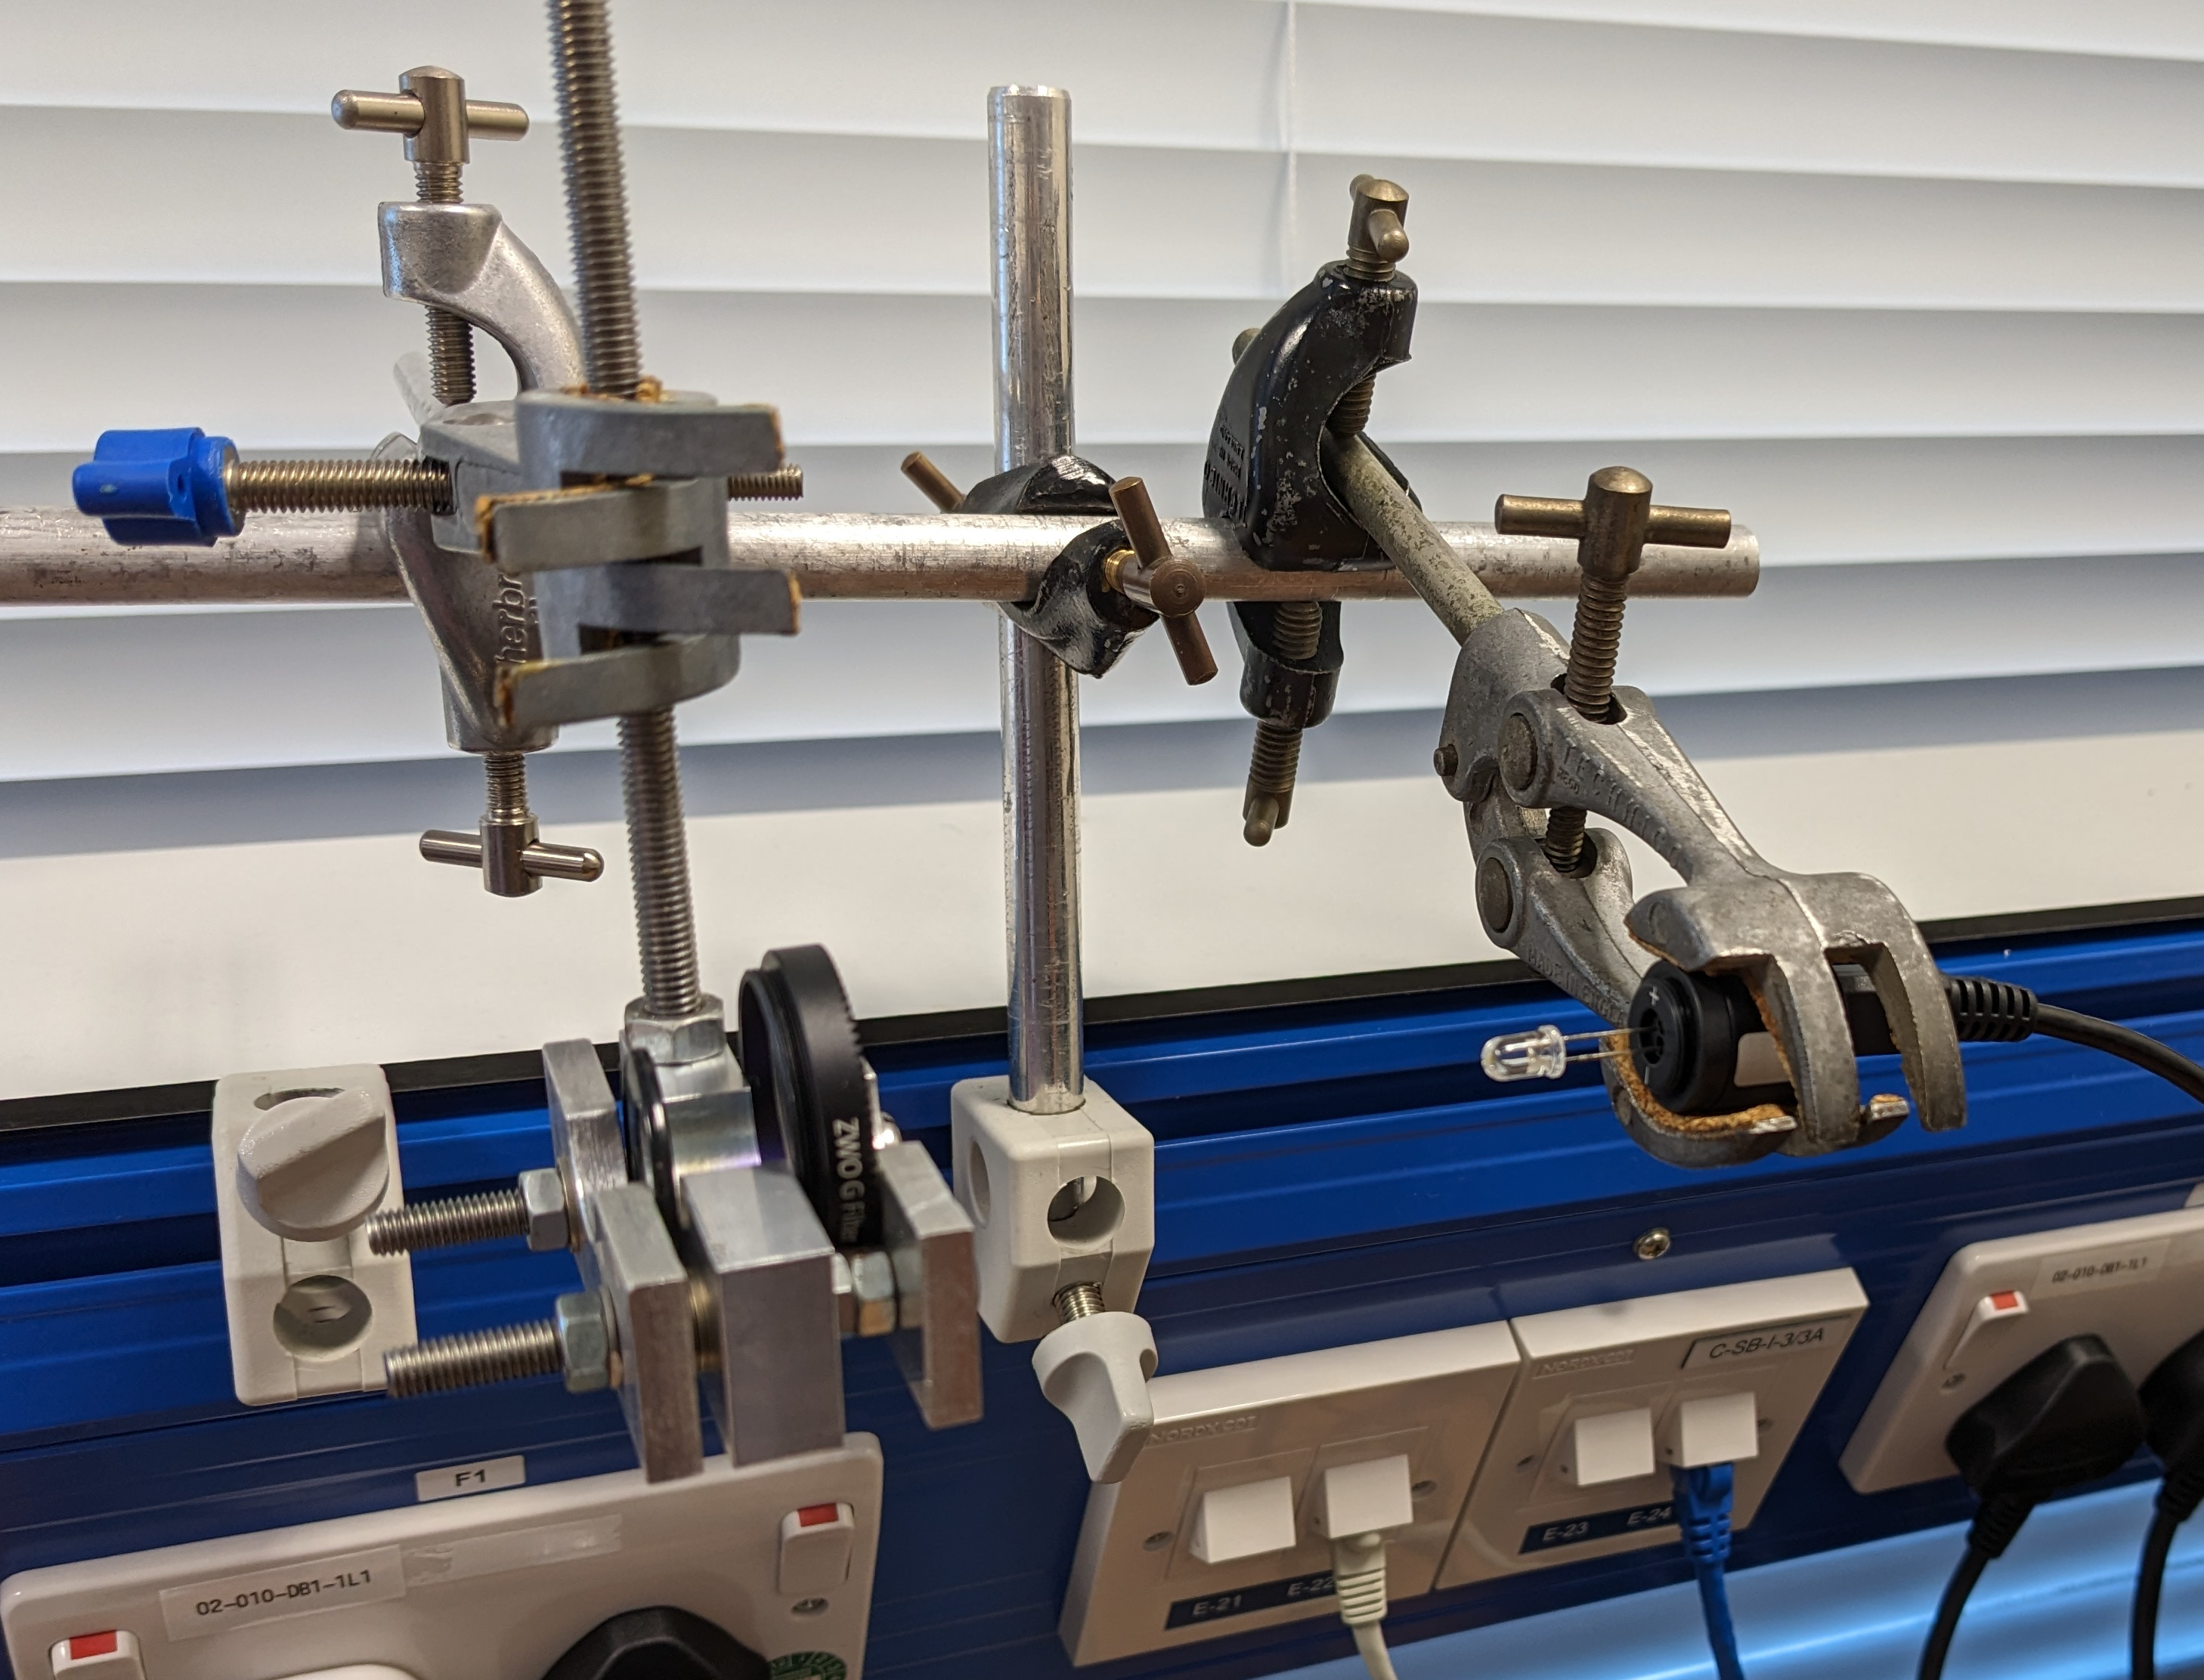
\includegraphics[width=0.8\textwidth]{doc/source_led.png}
    \includegraphics[width=0.8\textwidth]{doc/source.png}
    \caption{Light source, aperture, and filter setups. Both USB and bike light are mounted the same way, with the USB plugged into a nearby computer. The filter and aperture token holder is at the left, and a clamp on the right holds the light source.}
    \label{fig:source}
\end{figure}

\begin{figure}[h]
    \centering
    \includegraphics[width=0.49\textwidth]{doc/source1.png}
    \includegraphics[width=0.49\textwidth]{doc/source2.png}
    \includegraphics[width=0.49\textwidth]{doc/source3.png}
    \includegraphics[width=0.49\textwidth]{doc/source4.png}
    \caption{Example setup images. The top left is the light source, top right is light source on an misaligned with the aperture (note how the bright part of the source is offset from the aperture hole), bottom left is aligned with the token, and bottom right is with two filters to verify that the aperture is uniformly illuminated in a non-saturated image. For either light source, obtaining images like the lower right is the most important thing.}
    \label{fig:img_setup}
\end{figure}


\clearpage

\section{Software extras}

\subsection{\texttt{widget.py} in an ipython terminal}\label{sec:widget_ipython}

To run \texttt{widget.py} in a python terminal, you first need to open a terminal, specifically the \texttt{WinPython PowerShell Prompt}. This will probably not open in the folder you want, so navigate to your data using the \texttt{cd} command. When you are at or near your data, run \texttt{ipython}, which will start a python terminal.

With the \texttt{python} terminal running, you will need to import and then run the code. To import, you need to add the widget location to your path, which if you can do with (adjusting the path as necessary).
\begin{verbatim}
    import os, sys
    sys.path.append(os.path.abspath(`C:/px-interferometry'))
\end{verbatim}
You can then import and run the widget with
\begin{verbatim}
    import widget
    widget.fit_fringes(`Data/FOLDERS/file.FIT',sc=2)
\end{verbatim}
where you will need to enter the correct path to the file you want to extract the visibility for. The option \texttt{sc=2} is the same as the final argument described above.

\subsection{Jupyter notebook on lab ITS machines}\label{sec:jupyter_its}

To run a jupyter notebook on the lab ITS machines, open a `WinPython Powershell Prompt' from the interferometry-specific \texttt{WinPython} install in \texttt{C:}, change directory to \texttt{H:} with \texttt{cd H:}, and run \texttt{jupyter notebook}. A browser window should open, with which you can navigate to the downloaded notebooks.

\clearpage

\section{Troubleshooting}

\subsection{General}

\begin{itemize}
    \item Non-circular PSF: if you find that images are hard to fit and the PSF looks non-circular, it may be that the baseline token has some dust or other obscuration in one of both of the holes. This can be fixed by blowing, or (gently) pushing a pin or drillbit through the hole to clear it.
\end{itemize}

\subsection{Software}

\begin{itemize}
    \item To install software in \texttt{C:} on the lab computers one needs to create a new folder and put the software in there. This gets around permission issues. Each machine near a telescope should have \texttt{FireCapture} and \texttt{WinPython} installed.

    \item The default \texttt{WinPython} that appears in \texttt{C:} does not have the necessary packages (i.e. astropy, emcee). If necessary download a new one from \href{https://winpython.github.io/}{https://winpython.github.io/}. For the most recent release, click the Github download link (not a beta release), scroll to the bottom of the page, and download a version with a name like \texttt{WinPython64-X} (not a beta release indicated by a `b').

    \item To use \texttt{FireCapture} with the CMOS detector, the drivers need to be installed. These can be found in Software Center.
\end{itemize}

\clearpage

\bibliographystyle{aasjournal}
\bibliography{refs}

\end{document}  